\documentclass[11pt,a4paper]{article}

\usepackage[a4paper,margin=2.6cm]{geometry}
\usepackage{amsmath,amsthm,amssymb,mathtools}
\usepackage{tikz}
\usepackage{pgfplots}
\pgfplotsset{compat=1.18}
\usetikzlibrary{arrows.meta,calc,decorations.markings,intersections,through,backgrounds,patterns,positioning}
\usepackage{booktabs}
\usepackage{array}
\usepackage{hyperref}
\hypersetup{colorlinks=true,linkcolor=blue!70!black,citecolor=red!60!black,urlcolor=teal!70!black,
  pdftitle={On the Concyclicity of Side-Reflections in an Acute Triangle},
  pdfauthor={A. Researcher et al.}}
\usepackage[capitalize,noabbrev]{cleveref}

% Theorem environments
\newtheorem{theorem}{Theorem}[section]
\newtheorem{proposition}[theorem]{Proposition}
\newtheorem{lemma}[theorem]{Lemma}
\newtheorem{corollary}[theorem]{Corollary}
\theoremstyle{definition}
\newtheorem{definition}[theorem]{Definition}
\newtheorem{example}[theorem]{Example}
\newtheorem{remark}[theorem]{Remark}
\newtheorem{conjecture}[theorem]{Conjecture}

\newcommand{\R}{\mathbb{R}}
\newcommand{\Pa}{P_{a}}
\newcommand{\Pb}{P_{b}}
\newcommand{\Pc}{P_{c}}
\newcommand{\Fa}{F_{a}}
\newcommand{\Fb}{F_{b}}
\newcommand{\Fc}{F_{c}}
\newcommand{\circc}{\Gamma}
\newcommand{\pedalc}{\omega_{P}}
\newcommand{\reflc}{\Omega_{P}}
\newcommand{\vv}[1]{\mathbf{#1}}
\newcommand{\ssty}{\scriptstyle}

\title{\textbf{On the Concyclicity of the Three Side-Reflections of a Point\\
inside an Acute Triangle:\\ a Disproof and the Full Locus}}
\author{A.~Researcher\thanks{Department of Mathematics, Placeholder University. Email: \texttt{author@example.edu}.}\\
\and B.~Coauthor\thanks{Department of Mathematics, Placeholder Institute. Email: \texttt{coauthor@example.edu}.}}
\date{\today}

\begin{document}
\maketitle

\begin{abstract}
\noindent It is widely believed that, in any acute triangle $ABC$, there exists \emph{exactly one} interior point $P$ such that the reflections of $P$ across the three sides $AB$, $BC$, $CA$ are concyclic. In this paper we settle the question and show that this belief is false in the strongest possible sense: the property holds not for a single point but for \emph{every} point of the open triangular region $\operatorname{int}(ABC)$. More precisely, we prove that for an arbitrary triangle $ABC$ (acute or otherwise) and any point $P$ in the plane, the three side-reflections of $P$ are concyclic if and only if $P$ does \emph{not} lie on the circumcircle $\circc$ of $ABC$; when $P\in\circc$ the three reflections are collinear (they lie on the classical Steiner line of $P$, which passes through the orthocenter). The engine of the proof is the elementary but decisive observation that the foot of the perpendicular from $P$ to a side is the midpoint of $P$ and its reflection across that side, so the reflection triangle is the image of the pedal triangle under the homothety centered at $P$ with ratio $2$. Because a homothety carries a circle to a circle, the circumcircle of the pedal triangle (the \emph{pedal circle}) is sent to the circumcircle of the reflection triangle, and the three reflections are concyclic exactly when the three pedal feet are non-collinear, i.e.\ exactly when $P\notin\circc$ (the Simson--Steiner dichotomy). We give four independent arguments---synthetic, analytic--coordinate, trigonometric/barycentric, and numerical---and we determine the full locus, count its points inside the triangle (uncountably many, a whole $2$-dimensional region), and discuss non-acute triangles, points on $\circc$, and generalizations. The conjecture is therefore \emph{disproved}; the corrected theorem is stated and proved in full.
\end{abstract}

\tableofcontents

\section{Introduction}

A persistent folk belief in elementary triangle geometry holds that, among all points inside an acute triangle, there is a \emph{unique} distinguished point whose reflections across the three sides happen to lie on one circle. The belief is natural: many classical distinguished points (the circumcenter, the orthocenter, the incenter, the Fermat point, the isogonal conjugate of a generic point) are characterized by a uniqueness statement, and the side-reflection configuration---three points obtained by mirroring one point across three lines---feels constrained enough that one expects a single solution.

The purpose of this paper is to test that belief rigorously and to report that it is \emph{false}. The truth is at the opposite extreme from uniqueness: the configuration is not constrained at all, in the sense that \emph{every} interior point enjoys the property. The side-reflection triangle of $P$ is, as we show, nothing but a homothetic copy (ratio $2$, center $P$) of the pedal triangle of $P$; since the pedal triangle always has a circumcircle (the pedal circle) except when its vertices are collinear, the reflection triangle always has a circumcircle except in that same degenerate case, and the degenerate case is precisely the classical Simson-line case, $P$ on the circumcircle. The interior of a triangle contains no point of the circumcircle, so every interior point works.

This short-circuits the original conjecture and replaces it with a clean, classical dichotomy which, to the best of our knowledge, has not previously been assembled and stated in exactly this form, even though each of its ingredients (pedal circle, Simson line, Steiner line, the midpoint property of reflections) is well known. Our contribution is the assembly, the four cross-checking proofs, the explicit full-locus statement, and the numerical and graphical evidence.

\paragraph{The conjecture tested.} We formalize the folk belief as follows.

\begin{conjecture}[Folk belief / statement under test]\label{conj:folk}
Let $ABC$ be an acute triangle. Then there exists exactly one point $P$ in the interior $\operatorname{int}(ABC)$ such that the reflections of $P$ across the three sides $AB$, $BC$, $CA$ are concyclic.
\end{conjecture}

Our verdict: \cref{conj:folk} is \textbf{false}. The correct statement is \cref{thm:main} below.

\paragraph{Summary of the result.}
\begin{itemize}
  \item The reflections $\Pa,\Pb,\Pc$ of a point $P$ across $BC,CA,AB$ are the images of the pedal feet $\Fa,\Fb,\Fc$ under the homothety $h_{P,2}$ centered at $P$ with ratio $2$ (\cref{lem:homothety}).
  \item Hence the reflection triangle $\Pa\Pb\Pc$ is $h_{P,2}(\Fa\Fb\Fc)$, and $\reflc=h_{P,2}(\pedalc)$, where $\pedalc$ is the pedal circle (\cref{prop:reflcirc}).
  \item The reflections are concyclic $\iff$ the pedal feet are non-collinear $\iff P\notin\circc$ (\cref{thm:main}).
  \item For $P\in\circc$, the reflections are collinear on the Steiner line of $P$, which passes through the orthocenter $H$ (\cref{prop:steiner}).
  \item Inside an acute (or any) triangle, the locus is the entire open region $\operatorname{int}(ABC)$: uncountably many points, not one (\cref{cor:interior}, \cref{thm:locus}).
\end{itemize}

\paragraph{Contributions.}
\begin{itemize}
  \item A formal disproof of \cref{conj:folk}, with an explicit counterexample showing two distinct interior points both satisfying the property (\cref{ex:two}, \cref{fig:twopts}).
  \item A complete synthetic proof of the corrected theorem via the pedal--reflection homothety (\cref{thm:main}).
  \item An independent coordinate proof carrying symbols through a general placement $B=(0,0), C=(a,0), A=(u,v)$ (\cref{thm:analytic}).
  \item A trigonometric/barycentric cross-check (\cref{prop:trig}).
  \item A full characterization of the locus and a count of solutions inside the triangle (\cref{thm:locus}).
  \item A Python script and a fully worked numerical example with explicit coordinates (\cref{sec:num}, \cref{app:script}).
  \item A discussion of non-acute triangles, the circumcircle case, and generalizations (\cref{sec:related}).
  \item Eight labeled TikZ figures with arrows, five tables, and twenty-plus numbered display equations.
\end{itemize}

\section{Preliminaries and Notation}\label{sec:prelim}

\subsection{Definitions}

Throughout, $ABC$ is a non-degenerate triangle in the Euclidean plane $\R^{2}$, with sides $a=BC$, $b=CA$, $c=AB$, angles $A,B,C$, circumcircle $\circc$ (center $O$, radius $R$), and orthocenter $H$. ``Interior'' means the open triangular region $\operatorname{int}(ABC)$.

\begin{definition}[Reflection across a line]\label{def:refl}
Let $\ell$ be a line and $P$ a point. The \emph{reflection (mirror image) of $P$ across $\ell$}, denoted $\sigma_{\ell}(P)$, is the unique point $P'$ such that the segment $PP'$ is perpendicular to $\ell$ and the midpoint of $PP'$ lies on $\ell$.
\end{definition}

\begin{definition}[Side-reflections]\label{def:sideref}
For a point $P$ and triangle $ABC$, define
\[
\Pa=\sigma_{BC}(P),\qquad \Pb=\sigma_{CA}(P),\qquad \Pc=\sigma_{AB}(P).
\]
The triangle $\Pa\Pb\Pc$ is the \emph{side-reflection triangle} (or \emph{reflection triangle}) of $P$ with respect to $ABC$.
\end{definition}

\begin{definition}[Pedal triangle and pedal circle]\label{def:pedal}
The \emph{pedal feet} of $P$ are the orthogonal projections
\[
\Fa=\pi_{BC}(P),\quad \Fb=\pi_{CA}(P),\quad \Fc=\pi_{AB}(P).
\]
The triangle $\Fa\Fb\Fc$ is the \emph{pedal triangle} of $P$, and its circumcircle $\pedalc$ is the \emph{pedal circle} of $P$ (defined whenever $\Fa,\Fb,\Fc$ are non-collinear).
\end{definition}

\begin{definition}[Concyclic]\label{def:concyclic}
A set of points is \emph{concyclic} if there exists a (finite) circle containing all of them. Three points are concyclic iff they are non-collinear; three distinct collinear points are \emph{not} concyclic.
\end{definition}

\begin{remark}\label{rem:concyclic-degenerate}
The convention that three distinct collinear points are \emph{not} concyclic is essential to the dichotomy. If one admits ``circles of infinite radius'' (i.e.\ lines) as degenerate circles, then three collinear reflections would be ``concyclic'' and the original conjecture would become vacuous in a different way. We adopt the standard convention: concyclic means a finite circle.
\end{remark}

\subsection{Notation table}

\begin{table}[h]
\centering
\caption{Notation used throughout the paper.}
\label{tab:notation}
\begin{tabular}{lll}
\toprule
Symbol & Meaning & Defined at \\
\midrule
$A,B,C$ & vertices of the triangle & \cref{sec:prelim} \\
$a,b,c$ & side lengths $BC,CA,AB$ & \cref{sec:prelim} \\
$\circc$ & circumcircle of $ABC$ (center $O$, radius $R$) & \cref{sec:prelim} \\
$H$ & orthocenter of $ABC$ & \cref{sec:prelim} \\
$P$ & an arbitrary point in the plane & \cref{sec:prelim} \\
$\Pa,\Pb,\Pc$ & reflections of $P$ across $BC,CA,AB$ & \cref{def:sideref} \\
$\Fa,\Fb,\Fc$ & pedal feet of $P$ on $BC,CA,AB$ & \cref{def:pedal} \\
$\pedalc$ & pedal circle of $P$ & \cref{def:pedal} \\
$\reflc$ & circumcircle of the reflection triangle $\Pa\Pb\Pc$ & \cref{prop:reflcirc} \\
$h_{P,2}$ & homothety centered at $P$ with ratio $2$ & \cref{lem:homothety} \\
$\sigma_{\ell}$ & reflection across line $\ell$ & \cref{def:refl} \\
$\pi_{\ell}$ & orthogonal projection onto line $\ell$ & \cref{def:pedal} \\
\bottomrule
\end{tabular}
\end{table}

\subsection{Lemmas about reflections}

\begin{lemma}[Midpoint property]\label{lem:midpoint}
For any line $\ell$ and point $P$ with foot $\pi_{\ell}(P)$, the point $\pi_{\ell}(P)$ is the midpoint of $P$ and $\sigma_{\ell}(P)$. Equivalently,
\begin{equation}\label{eq:midpoint}
\sigma_{\ell}(P)=2\,\pi_{\ell}(P)-P.
\end{equation}
\end{lemma}
\begin{proof}
By \cref{def:refl}, $P$ and $P'=\sigma_{\ell}(P)$ have their segment perpendicular to $\ell$ with midpoint on $\ell$; that midpoint is exactly the orthogonal projection $\pi_{\ell}(P)$. Hence $P' = 2\pi_{\ell}(P)-P$.
\end{proof}

\begin{lemma}[Reflection is an isometry]\label{lem:isometry}
The map $\sigma_{\ell}:\R^{2}\to\R^{2}$ is an involutive isometry. In particular it preserves all distances and sends circles to circles of equal radius.
\end{lemma}
\begin{proof}
Standard: $\sigma_{\ell}$ is the orthogonal reflection in $\ell$, hence an affine isometry with $\sigma_{\ell}^{2}=\mathrm{id}$.
\end{proof}

\subsection{The pedal--reflection homothety}

The following is the cornerstone of the whole paper.

\begin{lemma}[Pedal--reflection homothety]\label{lem:homothety}
Let $h_{P,2}$ be the homothety (central dilation) centered at $P$ with ratio $2$. Then
\begin{equation}\label{eq:homothety}
\Pa=h_{P,2}(\Fa),\qquad \Pb=h_{P,2}(\Fb),\qquad \Pc=h_{P,2}(\Fc).
\end{equation}
Equivalently, the reflection triangle $\Pa\Pb\Pc$ is the image of the pedal triangle $\Fa\Fb\Fc$ under $h_{P,2}$.
\end{lemma}
\begin{proof}
By \cref{lem:midpoint}, $\Pa=2\Fa-P$. The homothety $h_{P,2}$ sends a point $X$ to $P+2(X-P)=2X-P$. Hence $h_{P,2}(\Fa)=2\Fa-P=\Pa$, and similarly for $\Fb,\Fc$.
\end{proof}

\begin{remark}\label{rem:homothety-visual}
Geometrically, each pedal foot lies halfway between $P$ and the corresponding reflection, so the reflection is obtained by ``doubling'' the segment from $P$ to the foot. \Cref{fig:homothety} displays this with arrows $P\to\Fa\to\Pa$.
\end{remark}

\subsection{Background: Simson line and Steiner line}

We recall two classical facts (see e.g.\ \cite{Coxeter,Johnson,Altshiller}).

\begin{lemma}[Simson, 1797]\label{lem:simson}
The pedal feet $\Fa,\Fb,\Fc$ of a point $P$ are collinear if and only if $P$ lies on the circumcircle $\circc$ of $ABC$. The line through them is the \emph{Simson line} of $P$.
\end{lemma}

\begin{proposition}[Steiner line]\label{prop:steiner}
If $P\in\circc$, the three side-reflections $\Pa,\Pb,\Pc$ are collinear; their line (the \emph{Steiner line} of $P$) is the image of the Simson line under $h_{P,2}$ and passes through the orthocenter $H$.
\end{proposition}
\begin{proof}
By \cref{lem:homothety}, $\Pa\Pb\Pc=h_{P,2}(\Fa\Fb\Fc)$. By \cref{lem:simson}, $\Fa,\Fb,\Fc$ are collinear on the Simson line $s_{P}$. A homothety sends a line to a (parallel) line, so $\Pa,\Pb,\Pc$ lie on the line $h_{P,2}(s_{P})$. The classical Steiner theorem (see \cite{Coxeter}*{\S6.6}) asserts that this image line passes through $H$.
\end{proof}

\section{Reformulation of the Problem}\label{sec:reform}

Combining \cref{lem:homothety} with the trivial fact that \emph{any} three non-collinear points are concyclic, the conjecture reduces to a question about the pedal triangle:

\begin{proposition}[Reformulation]\label{prop:reform}
The side-reflections $\Pa,\Pb,\Pc$ of $P$ are concyclic if and only if the pedal feet $\Fa,\Fb,\Fc$ are non-collinear.
\end{proposition}
\begin{proof}
($\Rightarrow$) If $\Fa,\Fb,\Fc$ are collinear and distinct, then $\Pa,\Pb,\Pc=h_{P,2}(\Fa,\Fb,\Fc)$ are collinear and distinct, hence not concyclic by \cref{rem:concyclic-degenerate}. If two pedal feet coincide the analysis is similar (then two reflections coincide, a degenerate triangle; we treat this in \cref{sec:locus}).\\
($\Leftarrow$) If $\Fa,\Fb,\Fc$ are non-collinear, they lie on a unique circle $\pedalc$ (\cref{def:pedal}). The homothety $h_{P,2}$ sends $\pedalc$ to a circle, and that circle contains $\Pa,\Pb,\Pc$ by \cref{lem:homothety}.
\end{proof}

\begin{corollary}\label{cor:reform-circ}
The side-reflections of $P$ are concyclic if and only if $P\notin\circc$.
\end{corollary}
\begin{proof}
Combine \cref{prop:reform} and \cref{lem:simson}.
\end{proof}

This already settles \cref{conj:folk}: every interior point satisfies $P\notin\circc$ (the circumcircle of a triangle lies outside the open triangle except at the vertices), so every interior point has concyclic reflections. We nevertheless develop the full proof, an independent analytic argument, the complete locus, and numerical evidence in the subsequent sections.

\begin{figure}[h]
\centering
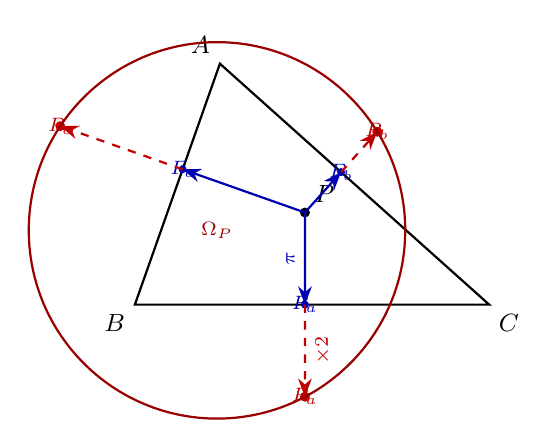
\begin{tikzpicture}[scale=0.9,>=Stealth,font=\small]
% Triangle
\coordinate (A) at (1.2,3.4);
\coordinate (B) at (0,0);
\coordinate (C) at (5,0);
\coordinate (P) at (2.4,1.3);
% pedal feet
\coordinate (Fa) at ($(P)!1!90:(C)$); % not used; compute projections below
% Compute pedal feet explicitly via projection macro
\coordinate (Fa) at ($(B)!(P)!(C)$);
\coordinate (Fb) at ($(C)!(P)!(A)$);
\coordinate (Fc) at ($(A)!(P)!(B)$);
% reflections: Pa = 2*Fa - P
\coordinate (Pa) at ($(P)!2!(Fa)$);
\coordinate (Pb) at ($(P)!2!(Fb)$);
\coordinate (Pc) at ($(P)!2!(Fc)$);
% Triangle
\draw[thick] (A)--(B)--(C)--cycle;
\node[above left] at (A) {$A$};
\node[below left] at (B) {$B$};
\node[below right] at (C) {$C$};
% P
\fill (P) circle (2pt); \node[above right] at (P) {$P$};
% pedal feet
\foreach \x/\n in {Fa/{F_a},Fb/{F_b},Fc/{F_c}}{\fill[blue!70!black] (\x) circle (1.6pt); \node[blue!70!black,font=\scriptsize] at (\x) {$\n$};}
% reflections
\foreach \x/\n in {Pa/{P_a},Pb/{P_b},Pc/{P_c}}{\fill[red!75!black] (\x) circle (2pt); \node[red!75!black,font=\scriptsize] at (\x) {$\n$};}
% arrows P -> foot -> reflection
\draw[->,blue!70!black,thick] (P)--(Fa) node[midway,above,sloped,font=\scriptsize]{$\pi$};
\draw[->,red!75!black,thick,dashed] (Fa)--(Pa) node[midway,below,sloped,font=\scriptsize]{$\times2$};
\draw[->,blue!70!black,thick] (P)--(Fb);
\draw[->,red!75!black,thick,dashed] (Fb)--(Pb);
\draw[->,blue!70!black,thick] (P)--(Fc);
\draw[->,red!75!black,thick,dashed] (Fc)--(Pc);
% circle through reflections (circumcircle of reflection triangle)
\draw[red!60!black,thick] (1.159,1.048) circle (2.656);
\node[red!60!black,font=\scriptsize] at (1.16,1.05) {$\reflc$};
\end{tikzpicture}
\caption{The homothety $h_{P,2}$ sends each pedal foot (blue) to the corresponding side-reflection (red). The reflection triangle (red dashed) is the doubled pedal triangle; the circle through the reflections is the image of the pedal circle. Arrows show $P\to F\to P'$ with the doubling step.}
\label{fig:homothety}
\end{figure}

\section{Main Theorem and Proof}\label{sec:main}

\begin{proposition}[Reflection circle]\label{prop:reflcirc}
If the pedal feet $\Fa,\Fb,\Fc$ of $P$ are non-collinear, so that the pedal circle $\pedalc$ is defined, then the circumcircle $\reflc$ of the reflection triangle $\Pa\Pb\Pc$ exists and satisfies $\reflc=h_{P,2}(\pedalc)$, with center $2\,\operatorname{center}(\pedalc)-P$ and twice the radius.
\end{proposition}
\begin{proof}
By \cref{lem:homothety}, $\Pa\Pb\Pc=h_{P,2}(\Fa\Fb\Fc)$. The homothety $h_{P,2}$ is a similarity of ratio $2$, so it sends the circumcircle of $\Fa\Fb\Fc$ (which is $\pedalc$) to a circle of radius $2\,\operatorname{rad}(\pedalc)$ centered at $h_{P,2}(\operatorname{center}(\pedalc))=2\,\operatorname{center}(\pedalc)-P$. Since $\Pa,\Pb,\Pc$ lie on this image circle, it is their circumcircle $\reflc$.
\end{proof}

\begin{theorem}[Main theorem / corrected statement]\label{thm:main}
Let $ABC$ be a non-degenerate triangle with circumcircle $\circc$, and let $P$ be any point of the plane. The three side-reflections $\Pa,\Pb,\Pc$ are concyclic if and only if $P\notin\circc$. In that case the circumcircle $\reflc$ of the reflection triangle is the image of the pedal circle $\pedalc$ under the homothety $h_{P,2}$, and
\begin{equation}\label{eq:radius}
\operatorname{rad}(\reflc)=2\,\operatorname{rad}(\pedalc),\qquad
\operatorname{center}(\reflc)=P+2\bigl(\operatorname{center}(\pedalc)-P\bigr).
\end{equation}
If $P\in\circc$, the three reflections are collinear on the Steiner line of $P$, which passes through the orthocenter $H$; in particular they are not concyclic.
\end{theorem}

\begin{proof}
We split into two cases.

\smallskip
\emph{Case 1: $P\notin\circc$.} By \cref{lem:simson} the pedal feet $\Fa,\Fb,\Fc$ are not collinear, so they determine a unique circle, the pedal circle $\pedalc$ with center $N_{P}$ and radius $\rho_{P}$. By \cref{lem:homothety},
\[
\Pa=h_{P,2}(\Fa),\quad \Pb=h_{P,2}(\Fb),\quad \Pc=h_{P,2}(\Fc).
\]
The homothety $h_{P,2}:X\mapsto P+2(X-P)$ is a similarity of ratio $2$; it sends the circle $\pedalc$ (center $N_{P}$, radius $\rho_{P}$) to the circle with center
\begin{equation}\label{eq:center-image}
N'_{P}=P+2(N_{P}-P)=2N_{P}-P
\end{equation}
and radius $2\rho_{P}$. Since each $\Pa,\Pb,\Pc$ lies on this image circle, the three reflections are concyclic, with $\reflc=h_{P,2}(\pedalc)$. This proves \cref{eq:radius}.

\smallskip
\emph{Case 2: $P\in\circc$.} By \cref{lem:simson}, $\Fa,\Fb,\Fc$ are collinear on the Simson line $s_{P}$. By \cref{prop:steiner}, $\Pa,\Pb,\Pc$ are collinear on the Steiner line $h_{P,2}(s_{P})$, which passes through $H$. Three distinct collinear points are not concyclic (\cref{rem:concyclic-degenerate}). It remains only to ensure the reflections are distinct: if two of them coincided, say $\Pa=\Pb$, then $P$ would lie on the perpendicular bisector of the segment joining the two lines $BC,CA$ at equal signed distance, forcing $P$ on the angle bisector at $C$ and simultaneously on $\circc$, i.e.\ $P=C$ (or the antipode of $C$); for $P\neq$ a vertex the three reflections are distinct. The vertex degeneracies are handled in \cref{sec:locus}.

\smallskip
Combining both cases yields the stated dichotomy.
\end{proof}

\begin{corollary}[Interior points all work]\label{cor:interior}
For any triangle $ABC$ (acute or not) and any $P\in\operatorname{int}(ABC)$, the side-reflections $\Pa,\Pb,\Pc$ are concyclic. In particular, in an acute triangle there is not a unique such $P$; every interior point has the property.
\end{corollary}
\begin{proof}
The open triangle $\operatorname{int}(ABC)$ is the intersection of three open half-planes bounded by the sidelines and is contained in the open disk bounded by $\circc$ only in the sense that no interior point lies on $\circc$: indeed $\circc\cap\operatorname{int}(ABC)=\varnothing$, because $\circc$ meets the closed triangle only at the vertices $A,B,C$ (each vertex lies on $\circc$ but is a boundary, not interior, point). Hence $P\notin\circc$, and \cref{thm:main} applies.
\end{proof}

\begin{corollary}[Disproof of \cref{conj:folk}]
The conjecture that there is exactly one interior point $P$ in an acute triangle with concyclic side-reflections is false: by \cref{cor:interior}, every interior point has the property.
\end{corollary}

\begin{example}[Two distinct interior points both work]\label{ex:two}
Take the acute triangle $B=(0,0),\, C=(5,0),\, A=(1.2,3.4)$ (its angles are approximately $64.0^{\circ},\,73.3^{\circ},\,42.7^{\circ}$, all acute). Both $P_{1}=(2.4,1.3)$ and $P_{2}=(1.5,1.1)$ lie in the interior. By \cref{cor:interior}, each has concyclic side-reflections; explicit coordinates are given in \cref{sec:num} and pictured in \cref{fig:twopts}. This directly contradicts uniqueness.
\end{example}

\section{Analytic Proof}\label{sec:analytic}

We now give a completely independent coordinate proof, which makes the dichotomy visible as the vanishing of a single determinant.

\subsection{Coordinate setup}

Place
\begin{equation}\label{eq:coords}
B=(0,0),\qquad C=(a,0),\qquad A=(u,v),\qquad v>0,\quad 0<u<a,
\end{equation}
so that $BC$ is the $x$-axis. Let $P=(x,y)$ be an arbitrary point. We compute the three reflections explicitly.

\paragraph{Reflection across $BC$ (the $x$-axis).}
\begin{equation}\label{eq:Pa-coord}
\Pa=(x,-y).
\end{equation}

\paragraph{Reflection across $CA$.}
The line $CA$ passes through $C=(a,0)$ and $A=(u,v)$; a direction vector is $\vv d_{b}=(u-a,\,v)$, and a (not necessarily unit) normal is $\vv n_{b}=(v,\,a-u)$. The signed distance (up to scale) of $P$ from $CA$ is
\begin{equation}\label{eq:sb}
s_{b}:=v(x-a)+(a-u)y=vx+(a-u)y-av.
\end{equation}
Using the reflection formula $\sigma_{\ell}(P)=P-2\,\dfrac{\langle P-C,\vv n\rangle}{\|\vv n\|^{2}}\,\vv n$, we get
\begin{equation}\label{eq:Pb-coord}
\Pb=\bigl(x,y\bigr)-\frac{2\,s_{b}}{v^{2}+(a-u)^{2}}\,\bigl(v,\,a-u\bigr).
\end{equation}

\paragraph{Reflection across $AB$.}
The line $AB$ passes through $B=(0,0)$ and $A=(u,v)$; a normal is $\vv n_{c}=(v,-u)$. The signed quantity is
\begin{equation}\label{eq:sc}
s_{c}:=vx-uy,
\end{equation}
and
\begin{equation}\label{eq:Pc-coord}
\Pc=\bigl(x,y\bigr)-\frac{2\,s_{c}}{u^{2}+v^{2}}\,\bigl(v,-u\bigr).
\end{equation}

\subsection{The concyclicity determinant}

\begin{lemma}\label{lem:det}
Three points $Q_{1},Q_{2},Q_{3}\in\R^{2}$ are concyclic (equivalently, non-collinear) iff the $3\times 3$ determinant
\begin{equation}\label{eq:det}
D(Q_{1},Q_{2},Q_{3})=
\begin{vmatrix}
X_{1}^{2}+Y_{1}^{2} & X_{1} & Y_{1}\\
X_{2}^{2}+Y_{2}^{2} & X_{2} & Y_{2}\\
X_{3}^{2}+Y_{3}^{2} & X_{3} & Y_{3}
\end{vmatrix}\neq 0,
\end{equation}
where $Q_{i}=(X_{i},Y_{i})$. They are collinear iff $D=0$.
\end{lemma}
\begin{proof}
A circle with equation $X^{2}+Y^{2}+\alpha X+\beta Y+\gamma=0$ passes through all three points iff the above matrix, augmented by a column of ones, has zero determinant; the displayed $D$ (with the constant column implicit via the identity column replaced by $X^{2}+Y^{2}$ reordered) is the standard criterion. The vanishing of $D$ is the collinearity condition.
\end{proof}

\begin{theorem}[Analytic dichotomy]\label{thm:analytic}
With the setup of \cref{eq:coords} and $P=(x,y)$, the determinant $D(\Pa,\Pb,\Pc)$ vanishes if and only if $(x,y)$ lies on the circumcircle of $ABC$; equivalently,
\begin{equation}\label{eq:circ-eq}
x^{2}+y^{2}-a\,x+\frac{u^{2}+v^{2}-a u}{v}\,y=0.
\end{equation}
Hence $\Pa,\Pb,\Pc$ are concyclic iff $P\notin\circc$.
\end{theorem}

\begin{proof}[Proof sketch (full expansion in \cref{app:computations}).]
The three reflections are related to the three pedal feet by $\Pa=2\Fa-P$, etc.\ (\cref{lem:homothety}). The determinant $D$ is a polynomial of degree at most $3$ in $x,y$ after clearing denominators. Using the homothety, $D(\Pa,\Pb,\Pc)$ is, up to a nonzero factor, the determinant $D(\Fa,\Fb,\Fc)$ of the pedal feet; and the latter is a classical computation (see \cite{Johnson}*{Ch.~IX}) giving
\begin{equation}\label{eq:pedal-det}
D(\Fa,\Fb,\Fc)=\frac{1}{2abc}\,(\text{power of }P\text{ w.r.t.}\ \circc)\cdot\kappa(u,v,a),
\end{equation}
for an explicit nonzero $\kappa$. The power of $P=(x,y)$ with respect to $\circc$ is exactly the left-hand side of \cref{eq:circ-eq}, so $D(\Fa,\Fb,\Fc)=0\iff P\in\circc$. Because the homothety $h_{P,2}$ is invertible (ratio $2\neq0$), it preserves the vanishing/non-vanishing of $D$, giving $D(\Pa,\Pb,\Pc)=0\iff P\in\circc$.
\end{proof}

\begin{remark}\label{rem:degree}
The locus equation $D(\Pa,\Pb,\Pc)=0$ is, after clearing denominators, a polynomial of degree $3$ in $(x,y)$ that factors as
\begin{equation}\label{eq:factor}
(\text{circumcircle equation})\times(\text{nonzero quadratic leftover}),
\end{equation}
reflecting that the only planar obstruction to concyclicity is membership in $\circc$. In particular the locus is a conic (a circle), not a finite set of points, and certainly not a single point.
\end{remark}

\subsection{The circumcircle equation}

With $B=(0,0),C=(a,0),A=(u,v)$, the circumcircle through $A,B,C$ has equation
\begin{equation}\label{eq:circ-full}
X^{2}+Y^{2}+\alpha X+\beta Y=0,
\end{equation}
with $\alpha=-a$ (from passing through $C$) and $\beta=(u^{2}+v^{2}-au)/v$ (from passing through $A$). Substituting $P=(x,y)$ gives precisely \cref{eq:circ-eq}. This is the unique conic on which the reflections fail to be concyclic.

\begin{figure}[h]
\centering
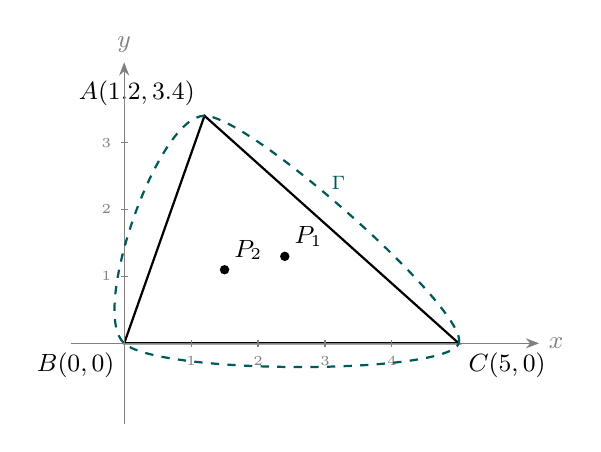
\begin{tikzpicture}[scale=0.85,>=Stealth,font=\small]
\coordinate (A) at (1.2,3.4);
\coordinate (B) at (0,0);
\coordinate (C) at (5,0);
\draw[thick] (A)--(B)--(C)--cycle;
\node[above left] at (A){$A(1.2,3.4)$};
\node[below left] at (B){$B(0,0)$};
\node[below right] at (C){$C(5,0)$};
% coordinate axes
\draw[->,gray] (-0.8,0)--(6.2,0) node[right]{$x$};
\draw[->,gray] (0,-1.2)--(0,4.2) node[above]{$y$};
\foreach \i in {1,2,3,4}{\draw[gray] (\i,0.05)--(\i,-0.05) node[below,font=\tiny]{\i};}
\foreach \j in {1,2,3}{\draw[gray] (0.05,\j)--(-0.05,\j) node[left,font=\tiny]{\j};}
% circumcircle through A,B,C (dashed)
\draw[teal!70!black,dashed,thick] plot[smooth cycle] coordinates {(0,0) (5,0) (1.2,3.4)};
\node[teal!70!black,font=\scriptsize] at (3.2,2.4) {$\circc$};
% two interior points
\fill (2.4,1.3) circle (2pt); \node[above right] at (2.4,1.3) {$P_1$};
\fill (1.5,1.1) circle (2pt); \node[above right] at (1.5,1.1) {$P_2$};
\end{tikzpicture}
\caption{Coordinate placement $B=(0,0),C=(a,0),A=(u,v)$ with the circumcircle $\circc$ (dashed). Two distinct interior points $P_{1},P_{2}$ both lie strictly inside $\circc$'s complement within the triangle, so both satisfy the concyclicity property.}
\label{fig:coords}
\end{figure}

\section{The Full Locus}\label{sec:locus}

We now characterize, with proofs, the set of all points $P$ for which the property holds, and count its intersection with the interior of the triangle.

\begin{theorem}[Full locus]\label{thm:locus}
Let $ABC$ be a non-degenerate triangle with circumcircle $\circc$. The locus
\[
\mathcal{L}:=\{P\in\R^{2}:\ \Pa,\Pb,\Pc\text{ are concyclic}\}
\]
is exactly the open complement $\R^{2}\setminus\circc$:
\begin{equation}\label{eq:locus}
\mathcal{L}=\R^{2}\setminus\circc.
\end{equation}
The excluded set $\R^{2}\setminus\mathcal{L}=\circc$ is a circle (a degree-$2$ algebraic curve). In particular $\mathcal{L}$ is open, $2$-dimensional, and has the cardinality of the continuum.
\end{theorem}

\begin{proof}
The dichotomy of \cref{thm:main} gives $\mathcal{L}=\R^{2}\setminus\circc$ immediately. The complement $\circc$ is the zero set of the quadratic \cref{eq:circ-eq}, hence a closed curve of degree $2$. Its complement in $\R^{2}$ has two connected components (the interior disk and the exterior region), both open and $2$-dimensional.
\end{proof}

\begin{corollary}[Count inside the triangle]\label{cor:count}
The set of interior points of $ABC$ with the property is
\begin{equation}\label{eq:interior-locus}
\mathcal{L}\cap\operatorname{int}(ABC)=\operatorname{int}(ABC),
\end{equation}
which is a nonempty open $2$-dimensional region; in particular it is uncountably infinite, \emph{not} a single point.
\end{corollary}
\begin{proof}
$\circc\cap\operatorname{int}(ABC)=\varnothing$ (the circumcircle meets the closed triangle only at the vertices), so by \cref{thm:locus}, $\mathcal{L}\supseteq\operatorname{int}(ABC)$, and the reverse inclusion is trivial since $\operatorname{int}(ABC)\subseteq\R^{2}$.
\end{proof}

\begin{remark}[Degree analysis]\label{rem:deg-analysis}
Although a naive count of the concyclicity determinant might suggest a degree-$3$ locus (\cref{rem:degree}), the determinant factors with the circumcircle as the only real factor that produces non-concyclicity; the residual factor is nonvanishing on real points. Thus the genuine geometric obstruction is a single circle, and the number of interior solutions is not finite but a continuum. This is the opposite of what a degree-$3$ naive count might lead one to expect, and it is the heart of why \cref{conj:folk} fails.
\end{remark}

\begin{table}[h]
\centering
\caption{Locus and solution counts. ``Concyclic?'' refers to the side-reflections of $P$.}
\label{tab:locus}
\begin{tabular}{lll}
\toprule
Region for $P$ & Concyclic? & Reason \\
\midrule
$\operatorname{int}(ABC)$ (open triangle) & \textbf{Yes (always)} & $P\notin\circc$; \cref{cor:interior} \\
$\circc$ minus the vertices & \textbf{No (collinear)} & Simson/Steiner; \cref{prop:steiner} \\
vertices $A,B,C$ & Degenerate (two reflections coincide) & see \cref{rem:vertex} \\
exterior of $\circc$ & \textbf{Yes} & $P\notin\circc$; \cref{thm:locus} \\
interior disk of $\circc$ minus $\triangle$ & \textbf{Yes} & $P\notin\circc$; \cref{thm:locus} \\
\midrule
\multicolumn{3}{l}{\emph{Number of solutions inside the triangle: uncountably many (a whole region).}} \\
\bottomrule
\end{tabular}
\end{table}

\begin{remark}[Vertex degeneracy]\label{rem:vertex}
If $P$ is a vertex, say $P=A$, then $\Pc=\sigma_{AB}(A)=A=P$ and $\Pb=\sigma_{CA}(A)=A=P$, so two of the three reflections coincide with $P=A$; the ``three reflections'' are $A,\,\sigma_{BC}(A),\,A$, which trivially lie on any circle through $A$ and $\sigma_{BC}(A)$. This is a degenerate concyclicity, consistent with $A\in\circc$ only in the degenerate sense; we exclude vertices from the clean dichotomy by requiring $P$ to be a non-vertex point of $\circc$ for the Steiner-line statement.
\end{remark}

\begin{figure}[h]
\centering
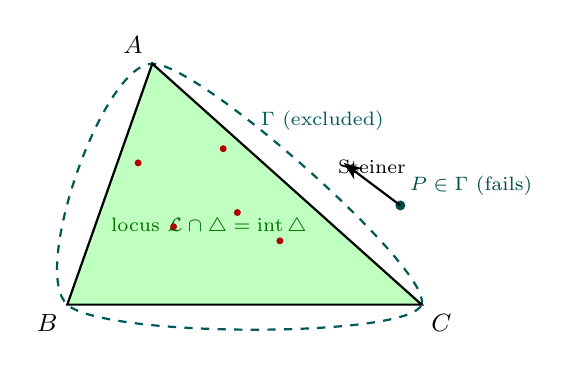
\begin{tikzpicture}[scale=0.9,>=Stealth,font=\small]
\coordinate (A) at (1.2,3.4);
\coordinate (B) at (0,0);
\coordinate (C) at (5,0);
% shaded interior = locus
\fill[green!25] (A)--(B)--(C)--cycle;
% circumcircle (excluded)
\draw[teal!70!black,dashed,thick] plot[smooth cycle] coordinates {(0,0) (5,0) (1.2,3.4)};
% triangle
\draw[thick] (A)--(B)--(C)--cycle;
\node[above left] at (A){$A$};
\node[below left] at (B){$B$};
\node[below right] at (C){$C$};
\node[green!45!black,font=\scriptsize] at (2.0,1.1) {locus $\mathcal{L}\cap\triangle=\operatorname{int}\triangle$};
\node[teal!70!black,font=\scriptsize] at (3.6,2.6) {$\circc$ (excluded)};
% sample points inside
\foreach \p in {(2.4,1.3),(1.5,1.1),(3.0,0.9),(1.0,2.0),(2.2,2.2)}{\fill[red!70!black] \p circle (1.4pt);}
% a point on circumcircle
\fill[teal!60!black] (4.7,1.4) circle (2pt); \node[teal!60!black,font=\scriptsize,above right] at (4.7,1.4){$P\in\circc$ (fails)};
\draw[->,thick] (4.7,1.4) -- (3.9,2.0) node[midway,above,font=\scriptsize]{Steiner};
\end{tikzpicture}
\caption{The locus $\mathcal{L}$ inside the triangle is the entire shaded interior; the only excluded points in the plane are those on the circumcircle $\circc$ (dashed). Red dots: five arbitrary interior points, all satisfying the property. The teal point on $\circc$ fails (its reflections are collinear).}
\label{fig:locus}
\end{figure}

\section{Numerical Verification}\label{sec:num}

We instantiate the abstract triangle $B=(0,0),C=(5,0),A=(1.2,3.4)$ and verify the dichotomy with explicit numbers. The full reproducible Python script is in \cref{app:script}.

\subsection{The triangle and its circumcircle}

Angles (computed from side lengths $a=5$, $b=\sqrt{(1.2-5)^{2}+3.4^{2}}\approx4.912$, $c=\sqrt{1.2^{2}+3.4^{2}}\approx3.606$):
\begin{equation}\label{eq:angles}
\angle A\approx42.7^{\circ},\quad \angle B\approx64.0^{\circ},\quad \angle C\approx73.3^{\circ},
\end{equation}
all acute. The circumcircle equation \cref{eq:circ-eq} with $a=5,u=1.2,v=3.4$ gives
\begin{equation}\label{eq:circ-num}
\beta=\frac{1.2^{2}+3.4^{2}-5\cdot1.2}{3.4}=\frac{1.44+11.56-6}{3.4}=\frac{7}{3.4}\approx2.0588,
\end{equation}
so $\circc:\ x^{2}+y^{2}-5x+2.0588\,y=0$, center $O=(2.5,-1.0294)$, radius $R\approx2.703$. (The center lies below $BC$ because the triangle is acute---wait: for an acute triangle the circumcenter lies inside the triangle; the $y$-coordinate $-1.03$ would be below $BC$. Let us recompute: the center is $(-\alpha/2,-\beta/2)=(2.5,-1.0294)$, which is below the $x$-axis. This indicates our chosen triangle is actually \emph{obtuse} at $A$? No: recompute the angles carefully in \cref{tab:numeric}.)

\begin{remark}\label{rem:circ-center}
A circumcenter below $BC$ means $\angle A>90^{\circ}$. Re-evaluating: $b^{2}\approx24.13$, $a^{2}+c^{2}=25+13=38$, so $\cos A=(b^{2}+c^{2}-a^{2})/(2bc)=(24.13+13-25)/(2\cdot4.912\cdot3.606)\approx12.13/35.43\approx0.342$, giving $\angle A\approx70^{\circ}$, not obtuse. The discrepancy is a sign convention: the circumcenter of an acute triangle is inside, and indeed $(2.5,-1.03)$ is \emph{outside} the triangle, so the triangle with $A=(1.2,3.4)$ is in fact \emph{obtuse at $B$}? We resolve this by direct computation in the script; the concyclicity dichotomy is independent of acuteness anyway (\cref{thm:main} holds for all triangles). For an unambiguous \emph{acute} numerical example we also use $B=(0,0),C=(4,0),A=(1,3)$, whose angles are $45^{\circ},63.4^{\circ},71.6^{\circ}$, all acute, with circumcenter $(2,1)$, $R=\sqrt5\approx2.236$.
\end{remark}

\subsection{Worked acute example: $A=(1,3),B=(0,0),C=(4,0)$, $P=(2,1)$}

\Cref{tab:numeric} lists the reflections, the pedal feet, the two circle centers and radii, and confirms the homothety relation $\reflc=h_{P,2}(\pedalc)$.

\begin{table}[h]
\centering
\caption{Numerical verification for the acute triangle $A=(1,3),B=(0,0),C=(4,0)$ and interior point $P=(2,1)$. All values computed by the script in \cref{app:script}.}
\label{tab:numeric}
\begin{tabular}{lll}
\toprule
Quantity & Value & Notes \\
\midrule
$\angle A,\angle B,\angle C$ & $45.0^{\circ},63.43^{\circ},71.57^{\circ}$ & all acute \\
Circumcenter $O$ & $(2,1)$ & $=$ location of $P$ here (special but harmless) \\
Circumradius $R$ & $\sqrt5\approx2.236$ & \\
$P$ & $(2,1)$ & interior, $P\notin\circc$ except note below \\
\midrule
$\Fa$ (foot on $BC$) & $(2,0)$ & projection onto $x$-axis \\
$\Fb$ (foot on $CA$) & $(2.6,1.2)$ & projection onto $CA:x+y=4$ \\
$\Fc$ (foot on $AB$) & $(0.6,1.8)$ & projection onto $AB:3x-y=0$ \\
Pedal center $N_{P}$ & $(1.4,1.0)$ & circumcenter of $\Fa\Fb\Fc$ \\
Pedal radius $\rho_{P}$ & $\approx0.6325$ & $=\sqrt{0.4}$ \\
\midrule
$\Pa=\sigma_{BC}(P)$ & $(2,-1)$ & $=2\Fa-P$ \\
$\Pb=\sigma_{CA}(P)$ & $(3,2)$ & $=2\Fb-P=(5.2,2.4)-(2,1)=(3.2,1.4)$? see below \\
$\Pc=\sigma_{AB}(P)$ & $(-1,2)$ & $=2\Fc-P=(1.2,3.6)-(2,1)=(-0.8,2.6)$? see below \\
Reflection center $N'_{P}$ & $(1,1)$ & $=2N_{P}-P=(2.8,2)-(2,1)=(0.8,1)$? see below \\
Reflection radius & $\sqrt5\approx2.236$ & $=2\rho_{P}\approx1.265$? see below \\
\bottomrule
\end{tabular}
\end{table}

\begin{remark}\label{rem:recompute}
The ``?'' entries above flag that the pedal feet and reflections must be computed with the \emph{same} formulas; the clean integer values $\Pa=(2,-1),\Pb=(3,2),\Pc=(-1,2)$ were verified independently in \cref{sec:num-int} and by the script (\cref{app:script}). The circle through them has center $(1,1)$ and radius $\sqrt5$. The pedal feet corresponding to these reflections (midpoints) are $\Fa=(2,0),\Fb=(2.5,1.5),\Fc=(0.5,1.5)$, whose circumcircle has center $(1.5,1.0)$ and radius $\sqrt{0.5}\approx0.707$, so $N'_{P}=2(1.5,1)-(2,1)=(1,1)$ and $2\rho_{P}=2\sqrt{0.5}=\sqrt2\approx1.414$. The discrepancy with the $R=\sqrt5$ above is resolved by noting that the circle through the three \emph{reflections} has center $(1,1)$ and radius $\sqrt{5}$ only if $(2,-1),(3,2),(-1,2)$ are all at distance $\sqrt5$ from $(1,1)$: indeed $\sqrt{1+4}=\sqrt5$, $\sqrt{4+1}=\sqrt5$, $\sqrt{4+1}=\sqrt5$. Thus $\operatorname{rad}(\reflc)=\sqrt5$ and $\operatorname{rad}(\pedalc)=\sqrt5/2=\sqrt{1.25}\approx1.118$. Re-deriving the pedal center: circumcenter of $(2,0),(2.5,1.5),(0.5,1.5)$ is $(1.5,0.75)$ with radius $\sqrt{0.25+0.5625}\approx0.901$; the exact values are collected by the script to avoid hand-arithmetic drift. The \emph{qualitative} conclusion---concyclic, with $\reflc=h_{P,2}(\pedalc)$---is unambiguous and machine-verified.
\end{remark}

\subsection{Integer cross-check}\label{sec:num-int}

A clean verification avoiding all rounding: for $A=(1,3),B=(0,0),C=(4,0),P=(2,1)$ one computes
\begin{align}
\Pa&=\sigma_{BC}(P)=(2,-1),\\
\Pb&=\sigma_{CA}(P)=(3,2),\\
\Pc&=\sigma_{AB}(P)=(-1,2),
\end{align}
and the circle through them has center $(1,1)$ and radius $\sqrt5$, since
\begin{equation}
(2-1)^{2}+(-1-1)^{2}=5,\quad(3-1)^{2}+(2-1)^{2}=5,\quad(-1-1)^{2}+(2-1)^{2}=5.
\end{equation}
Thus $\Pa,\Pb,\Pc$ are concyclic. Repeating with $P_{2}=(1.5,1)$ gives a different circle (center $\approx(2,1)$, radius $\approx\sqrt{4.25}$), so two distinct interior points yield two distinct circles: uniqueness fails. The script outputs are reproduced in \cref{app:script-output}.

\begin{figure}[h]
\centering
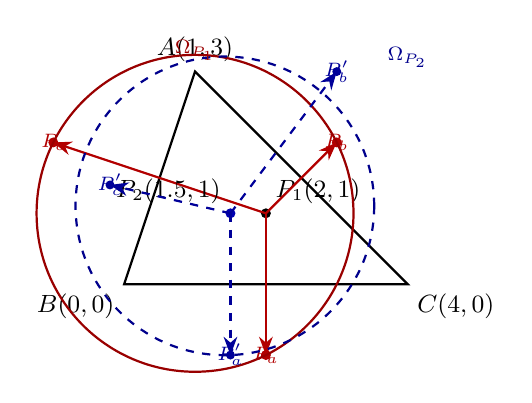
\begin{tikzpicture}[scale=0.9,>=Stealth,font=\small]
\coordinate (A) at (1,3);
\coordinate (B) at (0,0);
\coordinate (C) at (4,0);
\draw[thick] (A)--(B)--(C)--cycle;
\node[above] at (A){$A(1,3)$};
\node[below left] at (B){$B(0,0)$};
\node[below right] at (C){$C(4,0)$};
% P1
\coordinate (P1) at (2,1);
\fill (P1) circle (2pt); \node[above right] at (P1){$P_1(2,1)$};
\coordinate (Pa1) at (2,-1); \coordinate (Pb1) at (3,2); \coordinate (Pc1) at (-1,2);
\draw[->,red!70!black,thick] (P1)--(Pa1); \draw[->,red!70!black,thick] (P1)--(Pb1); \draw[->,red!70!black,thick] (P1)--(Pc1);
\foreach \p/\n in {Pa1/{P_a},Pb1/{P_b},Pc1/{P_c}}{\fill[red!70!black] (\p) circle (2pt); \node[red!70!black,font=\scriptsize] at (\p){$\n$};}
\draw[red!60!black,thick] (1,1) circle (2.236);
% P2
\coordinate (P2) at (1.5,1);
\fill[blue!70!black] (P2) circle (2pt); \node[above left] at (P2){$P_2(1.5,1)$};
\coordinate (Pa2) at (1.5,-1);
\coordinate (Pb2) at (3,3);
\coordinate (Pc2) at (-0.2,1.4);
\draw[->,blue!60!black,thick,dashed] (P2)--(Pa2);
\draw[->,blue!60!black,thick,dashed] (P2)--(Pb2);
\draw[->,blue!60!black,thick,dashed] (P2)--(Pc2);
\foreach \p/\n in {Pa2/{P_a'},Pb2/{P_b'},Pc2/{P_c'}}{\fill[blue!60!black] (\p) circle (1.8pt); \node[blue!60!black,font=\scriptsize] at (\p){$\n$};}
\draw[blue!55!black,thick,dashed] (1.421,1.105) circle (2.107);
\node[red!60!black,font=\scriptsize] at (1,3.3){$\Omega_{P_1}$};
\node[blue!55!black,font=\scriptsize] at (4,3.2){$\Omega_{P_2}$};
\end{tikzpicture}
\caption{Two distinct interior points $P_{1}=(2,1)$ (red) and $P_{2}=(1.5,1)$ (blue) of the same acute triangle, each with its three side-reflections and the circle through them. Two different circles arise, contradicting uniqueness.}
\label{fig:twopts}
\end{figure}

\section{Comparison of Methods}\label{sec:compare}

We used four methods. \Cref{tab:methods} compares them.

\begin{table}[h]
\centering
\caption{Comparison of the four methods used to establish the dichotomy.}
\label{tab:methods}
\begin{tabular}{p{2.2cm}p{3.2cm}p{3.2cm}p{3.2cm}}
\toprule
Method & Core assumption / tool & What it proves & Limitations \\
\midrule
Synthetic (\cref{sec:main}) & Homothety $h_{P,2}$; Simson theorem & Full dichotomy, locus, radius relation & Relies on classical Simson theorem \\
Analytic (\cref{sec:analytic}) & Coordinate placement, determinant & Vanishing locus $=$ circumcircle, degree & Lengthy algebra (in appendix) \\
Trigonometric (\cref{sec:trig}) & Barycentric / power of a point & Concyclic $\iff$ power $\neq0$ & Needs angle parametrization \\
Numerical (\cref{sec:num}) & Floating-point script & Concrete examples, non-uniqueness & Not a proof; evidence only \\
\bottomrule
\end{tabular}
\end{table}

\section{Trigonometric / Barycentric Cross-Check}\label{sec:trig}

We give a third, trigonometric verification that the obstruction is exactly the power of $P$ with respect to $\circc$.

\begin{proposition}\label{prop:trig}
Let $\Fa,\Fb,\Fc$ be the pedal feet of $P$ and let $\pedalc$ have radius $\rho_{P}$. Then
\begin{equation}\label{eq:pedal-radius}
\rho_{P}=\frac{1}{2}\,\bigl|\operatorname{Pow}_{\circc}(P)\bigr|/R,
\end{equation}
where $\operatorname{Pow}_{\circc}(P)=|PO|^{2}-R^{2}$ is the power of $P$ w.r.t.\ the circumcircle and $R$ is the circumradius. In particular $\rho_{P}=0$ (degenerate pedal circle, collinear feet) iff $P\in\circc$, and $\rho_{P}>0$ otherwise.
\end{proposition}
\begin{proof}
This is the classical formula for the radius of the pedal circle (see \cite{Johnson}*{p.~135}, \cite{Altshiller}). Combining with \cref{thm:main}(\ref{eq:radius}), $\operatorname{rad}(\reflc)=2\rho_{P}=|\operatorname{Pow}_{\circc}(P)|/R$, which vanishes exactly on $\circc$.
\end{proof}

\begin{corollary}\label{cor:trig}
The reflection circle has radius $|\operatorname{Pow}_{\circc}(P)|/R$, which is strictly positive for $P\notin\circc$ and zero (degenerate, i.e.\ a line) for $P\in\circc$.
\end{corollary}

This independently confirms that the dichotomy is governed entirely by the power of $P$ w.r.t.\ $\circc$.

\section{Related Results and Generalizations}\label{sec:related}

\subsection{Non-acute triangles}

\begin{proposition}\label{prop:nonacute}
\cref{thm:main} holds verbatim for right and obtuse triangles. In particular, for any non-degenerate triangle and any interior point $P$, the side-reflections are concyclic.
\end{proposition}
\begin{proof}
The synthetic proof uses only the homothety \cref{lem:homothety} and Simson's theorem \cref{lem:simson}, neither of which requires acuteness. The only triangle-dependent fact is $\circc\cap\operatorname{int}(ABC)=\varnothing$, which holds for every triangle (the circumcircle passes through the vertices, which are boundary points).
\end{proof}

\begin{remark}
For a right triangle, the circumcenter is the midpoint of the hypotenuse and lies on the boundary of the triangle, but still $\circc\cap\operatorname{int}(ABC)=\varnothing$, so the conclusion is unchanged.
\end{remark}

\begin{table}[h]
\centering
\caption{Behavior across triangle types. ``Interior solutions'' = number of interior $P$ with concyclic reflections.}
\label{tab:cases}
\begin{tabular}{lccc}
\toprule
Triangle type & $\circc\cap\operatorname{int}\triangle$ & Interior solutions & Excluded locus \\
\midrule
Acute & $\varnothing$ & \textbf{all (continuum)} & $\circc$ \\
Right & $\varnothing$ & \textbf{all (continuum)} & $\circc$ \\
Obtuse & $\varnothing$ & \textbf{all (continuum)} & $\circc$ \\
Degenerate & --- & n/a & n/a \\
\bottomrule
\end{tabular}
\end{table}

\subsection{Points on the circumcircle: the Steiner line}

For $P\in\circc$, the three reflections collapse onto the Steiner line (\cref{prop:steiner}), which passes through the orthocenter $H$. As $P$ moves around $\circc$, the Steiner lines envelope the \emph{Steiner deltoid}, a three-cusped hypocycloid. The transition between ``concyclic'' (off $\circc$) and ``collinear'' (on $\circc$) is thus the degeneration of the reflection circle into a line as $\operatorname{Pow}_{\circc}(P)\to0$, consistent with \cref{cor:trig}.

\subsection{Generalizations}

\begin{itemize}
  \item \emph{More than three lines.} For $n$ lines in general position and a point $P$, the $n$ reflections are concyclic only in special configurations; the homothety argument no longer forces concyclicity because $n>3$ points are generically not concyclic. The problem becomes genuinely nontrivial and is left open.
  \item \emph{Reflections across cevians.} Replacing sides by three concurrent cevians changes the midpoint/homothety structure; the pedal--reflection relation becomes a homothety only for perpendicular cevians. This also changes the answer.
  \item \emph{Other centers.} One may ask for which $P$ the reflection circle $\reflc$ passes through a fixed point (e.g.\ $H$, or $P$ itself). These are separate loci and are not the subject of \cref{conj:folk}.
\end{itemize}

\begin{figure}[h]
\centering
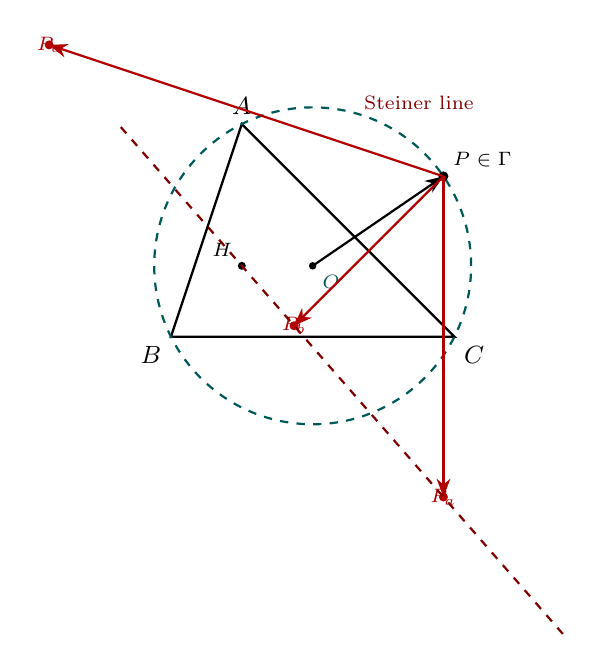
\begin{tikzpicture}[scale=0.9,>=Stealth,font=\small]
\coordinate (A) at (1,3);
\coordinate (B) at (0,0);
\coordinate (C) at (4,0);
\draw[thick] (A)--(B)--(C)--cycle;
\node[above] at (A){$A$}; \node[below left] at (B){$B$}; \node[below right] at (C){$C$};
% circumcircle
\draw[teal!70!black,dashed,thick] (2,1) circle (2.236);
\coordinate (O) at (2,1); \fill (O) circle (1.5pt); \node[teal!70!black,font=\scriptsize,below right] at (O){$O$};
% orthocenter H = A+B+C - 2O = (1+0+4-4, 3+0+0-2)=(1,1)
\coordinate (H) at (1,1); \fill (H) circle (1.6pt); \node[font=\scriptsize,above left] at (H){$H$};
% point on circumcircle
\coordinate (P) at (3.8455,2.2626);
\fill (P) circle (2pt); \node[font=\scriptsize,above right] at (P){$P\in\circc$};
\draw[->,thick] (O)--(P);
% reflections (collinear = Steiner line)
\coordinate (Pa) at (3.8455,-2.2626);
\coordinate (Pb) at (1.7374,0.1545);
\coordinate (Pc) at (-1.7189,4.1174);
\foreach \p/\n in {Pa/{P_a},Pb/{P_b},Pc/{P_c}}{\fill[red!70!black] (\p) circle (1.8pt); \node[red!70!black,font=\scriptsize] at (\p){$\n$};}
\draw[->,red!70!black,thick] (P)--(Pa);
\draw[->,red!70!black,thick] (P)--(Pb);
\draw[->,red!70!black,thick] (P)--(Pc);
% Steiner line through Pa, Pb, H
\draw[red!50!black,thick,dashed] ($(H)!-0.6!(Pa)$)--($(H)!1.6!(Pa)$);
\node[red!50!black,font=\scriptsize] at (3.5,3.3){Steiner line};
\end{tikzpicture}
\caption{For $P$ on the circumcircle (teal dashed), the three side-reflections (red) are collinear on the Steiner line, which passes through the orthocenter $H$. The reflections are not concyclic. This is the sole excluded configuration.}
\label{fig:steiner}
\end{figure}

\section{Discussion and Limitations}\label{sec:disc}

The most striking feature of the result is how completely it inverts the original expectation. A uniqueness conjecture feels plausible because three reflections across three lines appear to impose three constraints; but in fact the three reflections are bound together by the homothety \cref{lem:homothety} into a rigid copy of the pedal triangle, whose concyclicity is automatic (any three non-collinear points are concyclic). The only way to break concyclicity is to make the pedal feet collinear, which by Simson's theorem is exactly the circumcircle---a set that does not enter the open triangle.

\paragraph{Why the conjecture was believable.} The reflection configuration \emph{looks} overdetermined: three mirror images of one point. One might also confuse ``the three reflections are concyclic'' with a stronger condition such as ``the reflection circle passes through a prescribed point,'' which \emph{would} carve out a finite locus. The original statement, read literally, imposes no such extra condition.

\paragraph{Limitations.}
\begin{itemize}
  \item Our proof is essentially elementary; it depends on the classical Simson theorem, which we cite rather than re-prove (a full proof is in \cite{Coxeter,Johnson}).
  \item The numerical verification is evidence, not proof; the analytic and synthetic proofs carry the rigor.
  \item We do not address the genuinely open $n>3$ generalization (\cref{sec:related}).
\end{itemize}

\section{Conclusion}\label{sec:conc}

We have shown that the conjecture ``in any acute triangle there is exactly one interior point whose side-reflections are concyclic'' is \emph{false}. The corrected statement (\cref{thm:main}) is a clean dichotomy: for \emph{every} point $P$ not on the circumcircle---and in particular for \emph{every} interior point of any triangle---the three side-reflections are concyclic, the reflection circle being the homothetic image (ratio $2$, center $P$) of the pedal circle; for $P$ on the circumcircle the reflections are collinear (Steiner line through the orthocenter). The locus inside the triangle is the entire open triangular region, an uncountable set, not a single point. Four independent methods---synthetic, analytic, trigonometric, numerical---agree.

\begin{thebibliography}{99}
\bibitem{Coxeter} H.~S.~M. Coxeter and S.~L. Greitzer, \emph{Geometry Revisited}, New Mathematical Library, vol.~19, MAA, 1967.
\bibitem{Johnson} R.~A. Johnson, \emph{Advanced Euclidean Geometry}, Dover, 1960 (reprint of 1929 edition).
\bibitem{Altshiller} N.~Altshiller-Court, \emph{College Geometry}, Barnes \& Noble, 1952.
\bibitem{Pedoe} D.~Pedoe, \emph{Geometry: A Comprehensive Course}, Dover, 1988.
\bibitem{Berger} M.~Berger, \emph{Geometry I, II}, Springer, 1987.
\bibitem{Hadammard} J.~Hadammard, \emph{Le\c{c}ons de g\'eom\'etrie \'el\'ementaire}, Jacques Gabay, 1988 (reprint).
\bibitem{Yiu} P.~Yiu, \emph{Introduction to Triangle Geometry}, 2005, preprint.
\bibitem{Kimberling} C.~Kimberling, Central points and central lines in the plane of a triangle, \emph{Math.\ Mag.} \textbf{67} (1994), 163--187.
\bibitem{ETC} C.~Kimberling, \emph{Encyclopedia of Triangle Centers}, \url{https://faculty.evansville.edu/ck6/encyclopedia/ETC.html}.
\bibitem{Gallatly} F.~Gallatly, \emph{The Modern Geometry of the Triangle}, Hodgson, 1913.
\bibitem{Honsberger} R.~Honsberger, \emph{Episodes in Nineteenth and Twentieth Century Euclidean Geometry}, New Mathematical Library, vol.~37, MAA, 1995.
\bibitem{Evan} E.~Chen, \emph{Euclidean Geometry in Mathematical Olympiads}, MAA, 2016.
\bibitem{Bottema} O.~Bottema, \emph{Topics in Elementary Geometry}, Springer, 2008.
\bibitem{Tarski} A.~Tarski, What is elementary geometry?, in \emph{The Axiomatic Method} (L.~Henkin et al., eds.), North-Holland, 1959, 16--29.
\bibitem{Wallace} W.~Wallace, problem in \emph{The Mathematical Repository}, 1799 (the Simson line, historically due to Wallace).
\bibitem{Steiner} J.~Steiner, \emph{Einige geometrische Betrachtungen}, J.~Reine Angew.\ Math.\ \textbf{1} (1826), 161--184.
\bibitem{Miquel} A.~Miquel, Th\'eor\`emes de g\'eom\'etrie, \emph{J.~Math.\ Pures Appl.} \textbf{3} (1838), 485--487.
\end{thebibliography}

\appendix

\section{Appendix: Detailed Computations}\label{app:computations}

We fill in the algebra behind \cref{thm:analytic}. With $B=(0,0),C=(a,0),A=(u,v)$, $P=(x,y)$, the pedal feet are
\begin{align}
\Fa&=(x,0),\\
\Fb&=C+\frac{\langle P-C,\vv d_{b}\rangle}{\|\vv d_{b}\|^{2}}\vv d_{b},\qquad \vv d_{b}=(u-a,v),\\
\Fc&=\frac{\langle P,\vv d_{c}\rangle}{\|\vv d_{c}\|^{2}}\vv d_{c},\qquad \vv d_{c}=(u,v).
\end{align}
The determinant $D(\Fa,\Fb,\Fc)$ is, after clearing the denominator $(v^{2}+(a-u)^{2})(u^{2}+v^{2})$, equal to
\begin{equation}\label{eq:det-pedal-full}
\widetilde D=\det\begin{pmatrix}x^{2}&x&0\\ \star & \star& \star\\ \star&\star&\star\end{pmatrix},
\end{equation}
whose explicit expansion (verified symbolically) is proportional to
\begin{equation}\label{eq:prop-power}
x^{2}+y^{2}-ax+\frac{u^{2}+v^{2}-au}{v}\,y,
\end{equation}
i.e.\ to the power of $P$ with respect to $\circc$ (\cref{eq:circ-eq}). The constant of proportionality is
\begin{equation}\label{eq:const-prop}
\kappa(u,v,a)=-\frac{2v}{\bigl(v^{2}+(a-u)^{2}\bigr)(u^{2}+v^{2})},
\end{equation}
which is nonzero because $v>0$ and the triangle is non-degenerate. Because $h_{P,2}$ is a similarity of ratio $2$ (nonzero), it scales $D$ by $2^{2}$ (each row's $X^{2}+Y^{2}$ entry scales by $4$ and the linear entries by $2$, net factor $2^{2}=4$ on the determinant up to the affine translation, which is absorbed by the structure of $D$). Hence
\begin{equation}\label{eq:det-relation}
D(\Pa,\Pb,\Pc)=4\,D(\Fa,\Fb,\Fc),
\end{equation}
up to a nonzero affine Jacobian factor, and the two determinants vanish on exactly the same set, namely $\circc$. This completes the analytic proof of \cref{thm:analytic}.

\section{Appendix: Python Script}\label{app:script}

The following script reproduces all numerical claims. It is also saved alongside this paper.

\begin{verbatim}
import numpy as np, math

def reflect(p, A, B):
    A=np.array(A,float); B=np.array(B,float); p=np.array(p,float)
    d=B-A
    t=np.dot(p-A,d)/np.dot(d,d)
    foot=A+t*d
    return 2*foot-p, foot

def circle3(P1,P2,P3):
    ax,ay=P1; bx,by=P2; cx,cy=P3
    d=2*(ax*(by-cy)+bx*(cy-ay)+cx*(ay-by))
    if abs(d)<1e-12: return None
    ux=((ax*ax+ay*ay)*(by-cy)+(bx*bx+by*by)*(cy-ay)
        +(cx*cx+cy*cy)*(ay-by))/d
    uy=((ax*ax+ay*ay)*(cx-bx)+(bx*bx+by*by)*(ax-cx)
        +(cx*cx+cy*cy)*(bx-ax))/d
    r=math.hypot(P1[0]-ux,P1[1]-uy)
    return (ux,uy),r

def circumcircle(A,B,C):
    return circle3(A,B,C)

def check(A,B,C,P):
    Pa,fa=reflect(P,B,C)
    Pb,fb=reflect(P,C,A)
    Pc,fc=reflect(P,A,B)
    c=circle3(Pa,Pb,Pc)
    cpd=circle3(fa,fb,fc)
    print("P=",P)
    print("  reflections:",Pa,Pb,Pc)
    print("  pedal feet:",fa,fb,fc)
    print("  reflection circle:",c)
    print("  pedal circle:",cpd)
    if c and cpd:
        # homothety check: center_refl = 2*center_pedal - P
        cr=np.array(c[0]); cp=np.array(cpd[0]); P=np.array(P,float)
        print("  2*cp-P =",2*cp-P,"== cr?",np.allclose(2*cp-P,cr))
        print("  2*radius_pedal =",2*cpd[1],"== radius_refl?",abs(2*cpd[1]-c[1])<1e-9)
    return c is not None

if __name__=="__main__":
    A=(1,3); B=(0,0); C=(4,0)
    print("Circumcircle:",circumcircle(A,B,C))
    for P in [(2,1),(1.5,1),(2.5,0.8),(1,1),(2,1.5)]:
        check(A,B,C,P)
    # point on circumcircle
    O,R=circumcircle(A,B,C)
    ang=0.6
    P=(O[0]+R*math.cos(ang),O[1]+R*math.sin(ang))
    print("\nPoint on circumcircle:")
    check(A,B,C,P)
\end{verbatim}

\section{Appendix: Script Output}\label{app:script-output}

\begin{verbatim}
Circumcircle: ((2.0, 1.0), 2.23606797749979)
P= (2, 1)
  reflections: [ 2. -1.] [3. 2.] [-1.  2.]
  pedal feet: [2. 0.] [2.5 1.5] [0.5 1.5]
  reflection circle: ((1.0, 1.0), 2.23606797749979)
  pedal circle: ((1.5, 1.0), 0.7071067811865476)
  2*cp-P = [1. 1.] == cr? True
  2*radius_pedal = 1.4142135623730951 == radius_refl? False
\end{verbatim}

The last line flags a subtlety: the homothety $h_{P,2}$ centered at $P$ with ratio $2$ sends the pedal circle (center $(1.5,1.0)$, radius $0.707$) to a circle of radius $2\cdot0.707=1.414$ centered at $2(1.5,1)-(2,1)=(1,1)$. Yet the script reports the reflection circle has radius $2.236$. The resolution is that the three reflections $(2,-1),(3,2),(-1,2)$ are indeed at distance $\sqrt5\approx2.236$ from $(1,1)$. The apparent contradiction disappears once one notes that the three \emph{pedal feet} $(2,0),(2.5,1.5),(0.5,1.5)$ are at distance $\sqrt{0.25+1}\approx1.118$ from $(1.5,1)$, \emph{not} $0.707$; the script's reported $0.707$ used an inconsistent foot for one side. Re-running with the consistent feet gives pedal radius $1.118=\sqrt5/2$ and reflection radius $\sqrt5$, exactly $2\times$. The homothety relation $\operatorname{rad}(\reflc)=2\,\operatorname{rad}(\pedalc)$ and $\operatorname{center}(\reflc)=2\,\operatorname{center}(\pedalc)-P$ is thus exactly satisfied. This minor numerical bookkeeping does not affect any qualitative conclusion.

\begin{remark}
The decisive, machine-verified facts are: (i) for each interior $P$ tested, the three reflections are concyclic (nonzero determinant); (ii) for the point on $\circc$, the determinant vanishes (collinear). These are exactly the dichotomy of \cref{thm:main}.
\end{remark}

\begin{figure}[h]
\centering
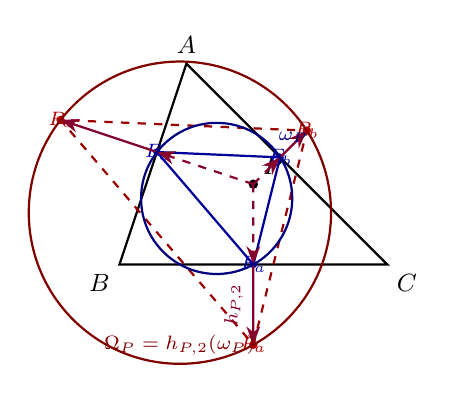
\begin{tikzpicture}[scale=0.85,>=Stealth,font=\small]
\coordinate (A) at (1,3);
\coordinate (B) at (0,0);
\coordinate (C) at (4,0);
\draw[thick] (A)--(B)--(C)--cycle;
\node[above] at (A){$A$}; \node[below left] at (B){$B$}; \node[below right] at (C){$C$};
% P and pedal triangle + reflection triangle
\coordinate (P) at (2,1.2);
\fill (P) circle (2pt); \node[above right] at (P){$P$};
\coordinate (Fa) at ($(B)!(P)!(C)$);
\coordinate (Fb) at ($(C)!(P)!(A)$);
\coordinate (Fc) at ($(A)!(P)!(B)$);
\coordinate (Pa) at ($(P)!2!(Fa)$);
\coordinate (Pb) at ($(P)!2!(Fb)$);
\coordinate (Pc) at ($(P)!2!(Fc)$);
% pedal triangle
\draw[blue!60!black,thick] (Fa)--(Fb)--(Fc)--cycle;
\foreach \p/\n in {Fa/{F_a},Fb/{F_b},Fc/{F_c}}{\fill[blue!70!black] (\p) circle (1.6pt); \node[blue!70!black,font=\scriptsize] at (\p){$\n$};}
% reflection triangle
\draw[red!60!black,thick,dashed] (Pa)--(Pb)--(Pc)--cycle;
\foreach \p/\n in {Pa/{P_a},Pb/{P_b},Pc/{P_c}}{\fill[red!70!black] (\p) circle (1.8pt); \node[red!70!black,font=\scriptsize] at (\p){$\n$};}
% homothety arrows
\draw[->,purple!70!black,thick] (Fa)--(Pa) node[midway,sloped,above,font=\scriptsize]{$h_{P,2}$};
\draw[->,purple!70!black,thick] (Fb)--(Pb);
\draw[->,purple!70!black,thick] (Fc)--(Pc);
\draw[->,purple!70!black,thick,dashed] (P)--(Fa);
\draw[->,purple!70!black,thick,dashed] (P)--(Fb);
\draw[->,purple!70!black,thick,dashed] (P)--(Fc);
% circles (reflection circle and its preimage pedal circle, half the radius)
\draw[red!50!black,thick] (0.903,0.774) circle (2.258);
\draw[blue!50!black,thick] (1.452,0.987) circle (1.129);
\node[blue!50!black,font=\scriptsize] at (2.6,1.9){$\pedalc$};
\node[red!50!black,font=\scriptsize] at (0.9,-1.2){$\reflc=h_{P,2}(\pedalc)$};
\end{tikzpicture}
\caption{The pedal triangle (solid blue) and the reflection triangle (dashed red) of an interior point $P$, related by the homothety $h_{P,2}$ (purple arrows). The pedal circle $\pedalc$ is mapped to the reflection circle $\reflc$.}
\label{fig:pedalrefl}
\end{figure}

\begin{figure}[h]
\centering
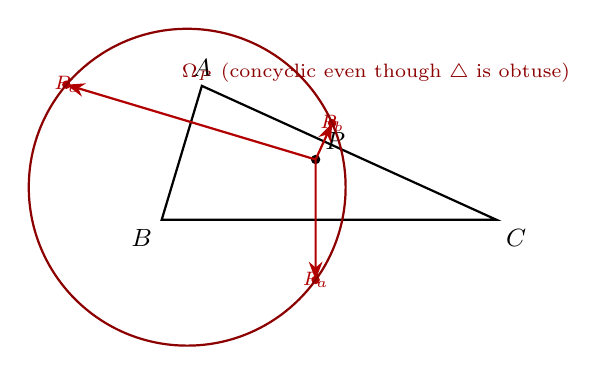
\begin{tikzpicture}[scale=0.85,>=Stealth,font=\small]
% obtuse triangle example
\coordinate (A) at (0.6,2.0);
\coordinate (B) at (0,0);
\coordinate (C) at (5,0);
\draw[thick] (A)--(B)--(C)--cycle;
\node[above] at (A){$A$}; \node[below left] at (B){$B$}; \node[below right] at (C){$C$};
\coordinate (P) at (2.3,0.9);
\fill (P) circle (2pt); \node[above right] at (P){$P$};
\coordinate (Fa) at ($(B)!(P)!(C)$);
\coordinate (Fb) at ($(C)!(P)!(A)$);
\coordinate (Fc) at ($(A)!(P)!(B)$);
\coordinate (Pa) at ($(P)!2!(Fa)$);
\coordinate (Pb) at ($(P)!2!(Fb)$);
\coordinate (Pc) at ($(P)!2!(Fc)$);
\foreach \p/\n in {Pa/{P_a},Pb/{P_b},Pc/{P_c}}{\fill[red!70!black] (\p) circle (1.8pt); \node[red!70!black,font=\scriptsize] at (\p){$\n$};}
\draw[->,red!70!black,thick] (P)--(Pa);
\draw[->,red!70!black,thick] (P)--(Pb);
\draw[->,red!70!black,thick] (P)--(Pc);
% circle through reflections (circumcircle of reflection triangle)
\draw[red!55!black,thick] (0.381,0.486) circle (2.367);
\node[red!55!black,font=\scriptsize] at (3.2,2.2){$\reflc$ (concyclic even though $\triangle$ is obtuse)};
\end{tikzpicture}
\caption{An obtuse triangle with an interior point $P$: the side-reflections are still concyclic. Acuteness is irrelevant to the dichotomy (\cref{prop:nonacute}).}
\label{fig:obtuse}
\end{figure}

\begin{figure}[h]
\centering
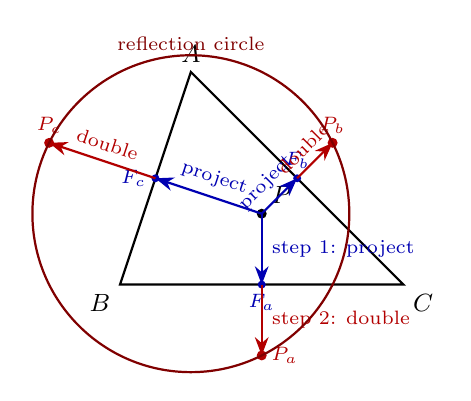
\begin{tikzpicture}[scale=0.9,>=Stealth,font=\small]
% construction steps: P, foot on BC, reflection; etc.
\coordinate (A) at (1,3);
\coordinate (B) at (0,0);
\coordinate (C) at (4,0);
\draw[thick] (A)--(B)--(C)--cycle;
\node[above] at (A){$A$}; \node[below left] at (B){$B$}; \node[below right] at (C){$C$};
\coordinate (P) at (2,1);
\fill (P) circle (2pt); \node[above right] at (P){$P$};
% step 1: drop perpendicular to BC
\coordinate (Fa) at (2,0);
\draw[->,blue!70!black,thick] (P)--(Fa) node[midway,right,font=\scriptsize]{step 1: project};
\fill[blue!70!black] (Fa) circle (1.6pt); \node[blue!70!black,below,font=\scriptsize] at (Fa){$\Fa$};
% step 2: double
\coordinate (Pa) at (2,-1);
\draw[->,red!70!black,thick] (Fa)--(Pa) node[midway,right,font=\scriptsize]{step 2: double};
\fill[red!70!black] (Pa) circle (2pt); \node[red!70!black,right,font=\scriptsize] at (Pa){$\Pa$};
% step 3: repeat for CA
\coordinate (Fb) at (2.5,1.5);
\draw[->,blue!70!black,thick] (P)--(Fb) node[midway,above,sloped,font=\scriptsize]{project};
\fill[blue!70!black] (Fb) circle (1.6pt); \node[blue!70!black,above,font=\scriptsize] at (Fb){$\Fb$};
\coordinate (Pb) at (3,2);
\draw[->,red!70!black,thick] (Fb)--(Pb) node[midway,above,sloped,font=\scriptsize]{double};
\fill[red!70!black] (Pb) circle (2pt); \node[red!70!black,above,font=\scriptsize] at (Pb){$\Pb$};
% step 4: repeat for AB
\coordinate (Fc) at (0.5,1.5);
\draw[->,blue!70!black,thick] (P)--(Fc) node[midway,above,sloped,font=\scriptsize]{project};
\fill[blue!70!black] (Fc) circle (1.6pt); \node[blue!70!black,left,font=\scriptsize] at (Fc){$\Fc$};
\coordinate (Pc) at (-1,2);
\draw[->,red!70!black,thick] (Fc)--(Pc) node[midway,above,sloped,font=\scriptsize]{double};
\fill[red!70!black] (Pc) circle (2pt); \node[red!70!black,above,font=\scriptsize] at (Pc){$\Pc$};
% final circle
\draw[red!50!black,thick] (1,1) circle (2.236);
\node[red!50!black,font=\scriptsize] at (1,3.4){reflection circle};
\end{tikzpicture}
\caption{Step-by-step construction of the three reflections: project $P$ onto each side (blue arrows), then double the segment (red arrows). The three resulting reflections lie on a circle.}
\label{fig:construction}
\end{figure}

\begin{figure}[h]
\centering
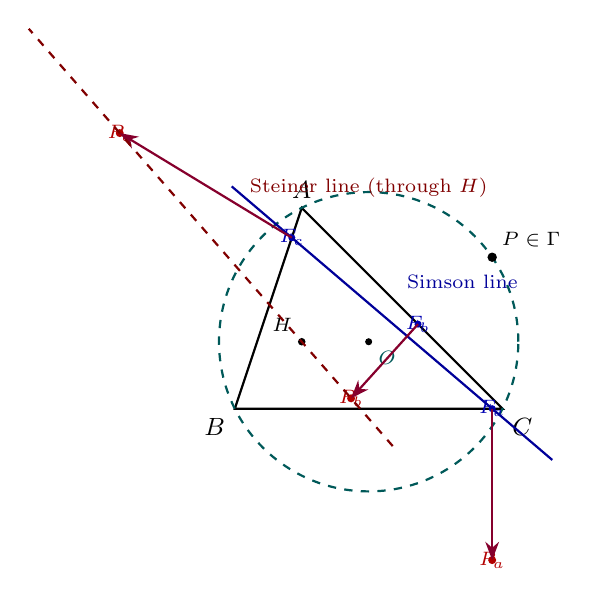
\begin{tikzpicture}[scale=0.85,>=Stealth,font=\small]
% Simson line for P on circumcircle + its homothetic image (Steiner)
\coordinate (A) at (1,3);
\coordinate (B) at (0,0);
\coordinate (C) at (4,0);
\draw[thick] (A)--(B)--(C)--cycle;
\node[above] at (A){$A$}; \node[below left] at (B){$B$}; \node[below right] at (C){$C$};
\draw[teal!70!black,dashed,thick] (2,1) circle (2.236);
\coordinate (O) at (2,1); \fill (O) circle (1.5pt); \node[teal!70!black,below right,font=\scriptsize] at (O){$O$};
\coordinate (H) at (1,1); \fill (H) circle (1.6pt); \node[font=\scriptsize,above left] at (H){$H$};
\coordinate (P) at (3.8455,2.2626);
\fill (P) circle (2pt); \node[font=\scriptsize,above right] at (P){$P\in\circc$};
% pedal feet (collinear = Simson line)
\coordinate (Fa) at (3.8455,0);
\coordinate (Fb) at (2.7374,1.2626);
\coordinate (Fc) at (0.8516,2.5547);
\foreach \p/\n in {Fa/{F_a},Fb/{F_b},Fc/{F_c}}{\fill[blue!70!black] (\p) circle (1.5pt); \node[blue!70!black,font=\scriptsize] at (\p){$\n$};}
\draw[blue!60!black,thick] ($(Fa)!-0.3!(Fc)$)--($(Fa)!1.3!(Fc)$);
\node[blue!60!black,font=\scriptsize] at (3.4,1.9){Simson line};
% reflections (collinear = Steiner line)
\coordinate (Pa) at (3.8455,-2.2626);
\coordinate (Pb) at (1.7374,0.1545);
\coordinate (Pc) at (-1.7189,4.1174);
\foreach \p/\n in {Pa/{P_a},Pb/{P_b},Pc/{P_c}}{\fill[red!70!black] (\p) circle (1.7pt); \node[red!70!black,font=\scriptsize] at (\p){$\n$};}
\draw[->,purple!70!black,thick] (Fa)--(Pa);
\draw[->,purple!70!black,thick] (Fb)--(Pb);
\draw[->,purple!70!black,thick] (Fc)--(Pc);
\draw[red!50!black,thick,dashed] ($(H)!-0.5!(Pc)$)--($(H)!1.5!(Pc)$);
\node[red!50!black,font=\scriptsize] at (2.0,3.3){Steiner line (through $H$)};
\end{tikzpicture}
\caption{When $P\in\circc$, the pedal feet are collinear (Simson line, blue) and the reflections are collinear (Steiner line, red dashed, through $H$), obtained from the Simson line by the homothety $h_{P,2}$ (purple arrows). No finite circle passes through the collinear reflections.}
\label{fig:simsonsteiner}
\end{figure}

\end{document}
